\documentclass[11pt,a4paper]{article}

\usepackage[utf8]{inputenc}
\usepackage[T1]{fontenc}
\usepackage[english]{babel}
\usepackage[margin=2.5cm]{geometry}
\usepackage{amsmath}
\usepackage{graphicx}
\usepackage{xcolor}
\usepackage{microtype}
\usepackage{authblk}
\usepackage[hidelinks]{hyperref}

% Items to confirm before submission, printed in red.
\newcommand{\ph}[1]{\textcolor{red!65!black}{[#1]}}

\title{Design of an Integrated VR-Biofeedback Framework for Controlled
Phobia Exposure}
\author[1]{Giorgio Mario Grasso}
\author[1]{Paria Daghooghi}
\author[1]{Yalda Asghari Dizaj}
\author[1]{Haleh Khorshidi}
\author[1]{Elaheh Bakhtiari}
\author[1]{Parsa Kazemi}
\author[1]{Erfan Zandi}
\author[1]{Benyamin Baharizadeh}
\author[2]{Febronia Riggio}
\author[2]{Carmelo Mario Porto}
\affil[1]{NISC Lab, Cognitive Science Department, University of Messina,
Italy}
\affil[2]{\ph{affiliation to be confirmed}}
\date{}

\begin{document}
\maketitle

\begin{center}
\small
Paper proposal, HCI International 2027, Berlin\\
Thematic area: \ph{Virtual, Augmented and Mixed Reality (VAMR), to be
confirmed}\\
Corresponding author: \ph{name and e-mail}\\
\ph{spelling of Haleh and Febronia to be confirmed}
\end{center}

\noindent\textbf{Keywords:} virtual reality, biofeedback, closed-loop
adaptation, electrodermal activity, heart-rate variability, phobia
exposure

\section*{Objective and significance}

Virtual reality can present feared situations, such as heights, under
experimental control, while wearable sensors follow the autonomic
response as it unfolds. In many virtual exposure systems the stimulus
follows a predefined progression, advanced by a script, an operator or
the participant~\cite{rothbaum1995,freeman2018}; physiology, where it is
recorded, informs later analysis rather than the environment. Systems
adapting the environment to physiological signals have shown that this
is
feasible~\cite{moldoveanu2023,kritikos2021,mahmoudinejad2021,wriessnegger2026}.
For such systems to be compared and replicated, measurement, decision
rule and environment must be fully specified and kept separable, so that
one calibrated index can drive different environments on identical
instrumentation. Our objective is a framework built on that principle.
The question belongs to human-computer interaction: how an interactive
system should read implicit physiological input and act on it in real
time while staying transparent, bounded and safe for the person inside
the loop.

\section*{Methods and approach}

The framework runs as a measurement server to which each virtual
environment connects as a client. A wireless biosignal unit
(biosignalsplux) records the electrocardiogram in a Lead~I configuration
from chest electrodes and skin conductance from two fingers of the
non-dominant hand, both at 1000~Hz, streamed over the Lab Streaming
Layer~\cite{kothe2025}. Heart rate over a 30~s window and RMSSD over a
60~s window~\cite{taskforce1996} are recomputed every 0.5~s, and the
phasic component of skin conductance~\cite{boucsein2012} is separated by
high-pass filtering, all with NeuroKit2~\cite{makowski2021}. A second,
independent implementation following the manufacturer's routines, and
replay of archived recordings through the live pipeline, allow derived
values to be checked on identical input.

Each session opens with a 120~s resting calibration after a settling
period. Every measure is standardised against its calibration
distribution: heart rate and RMSSD as percentage deviations from their
resting means, conductance as its phasic component, with RMSSD inverted
so that each term rises with arousal. The terms combine under
coefficients fixed in advance,
$S = 0.5\,z_{\mathrm{EDA}} + 0.3\,z_{\mathrm{HRV}} + 0.2\,z_{\mathrm{HR}}$,
and are smoothed by a 3~s trailing mean. Two thresholds, at the
calibration mean plus 1.28 and 2.33 standard deviations, divide the index
into three bands defined by the participant's own resting distribution.
The control law is deterministic: below the lower threshold the
environment is told to increase its stimulus, above the upper threshold
to decrease it, and between them nothing is sent. Commands are held at
the start of a run until the smoothed index first reads in the lowest
band, are limited to one per second, and stop while the sensor signal is
lost; a calibration that fails a validity check blocks the run.

The interface is scenario-neutral. Four command strings travel to the
environment over UDP, and telemetry returns in one JSON envelope whose
fields are recorded without being declared in advance. Each session
yields a 10~Hz record of signals, index and state, a diagnostic trace of
every raw value, the calibration parameters and a log of every command,
from which each run can be reconstructed. The first environment, built
in Unity~6 and shown on a Meta Quest headset, places the participant in a
hot-air balloon whose height each command raises or lowers. Two members
of the research team are present throughout, the participant may end the
session at any moment, and every participant gives written informed
consent under a protocol approved by \ph{ethics committee, protocol
number and date}.

\section*{Results and findings}

The framework is operational and in use in the laboratory. In the height
environment it has driven \ph{33} runs of about five minutes each, from
\ph{24} participants between July and September 2026, nine of whom
completed two sessions. Figure~\ref{fig:session} shows one of these runs:
over 312~s the system sent 98 \texttt{increase} and 123
\texttt{decrease} commands, and the balloon rose and fell twice between
15 and 80~m as the index crossed its thresholds. The full paper will give
the complete specification and operational figures across the recorded
set: completed calibrations, run durations, the balance of commands and
episodes of signal loss. Data collection continues. Effects on
self-reported fear are outside the scope of this paper and will be
reported separately.

\begin{figure}[tbp]
    \centering
    \IfFileExists{07-session-overview.png}{%
        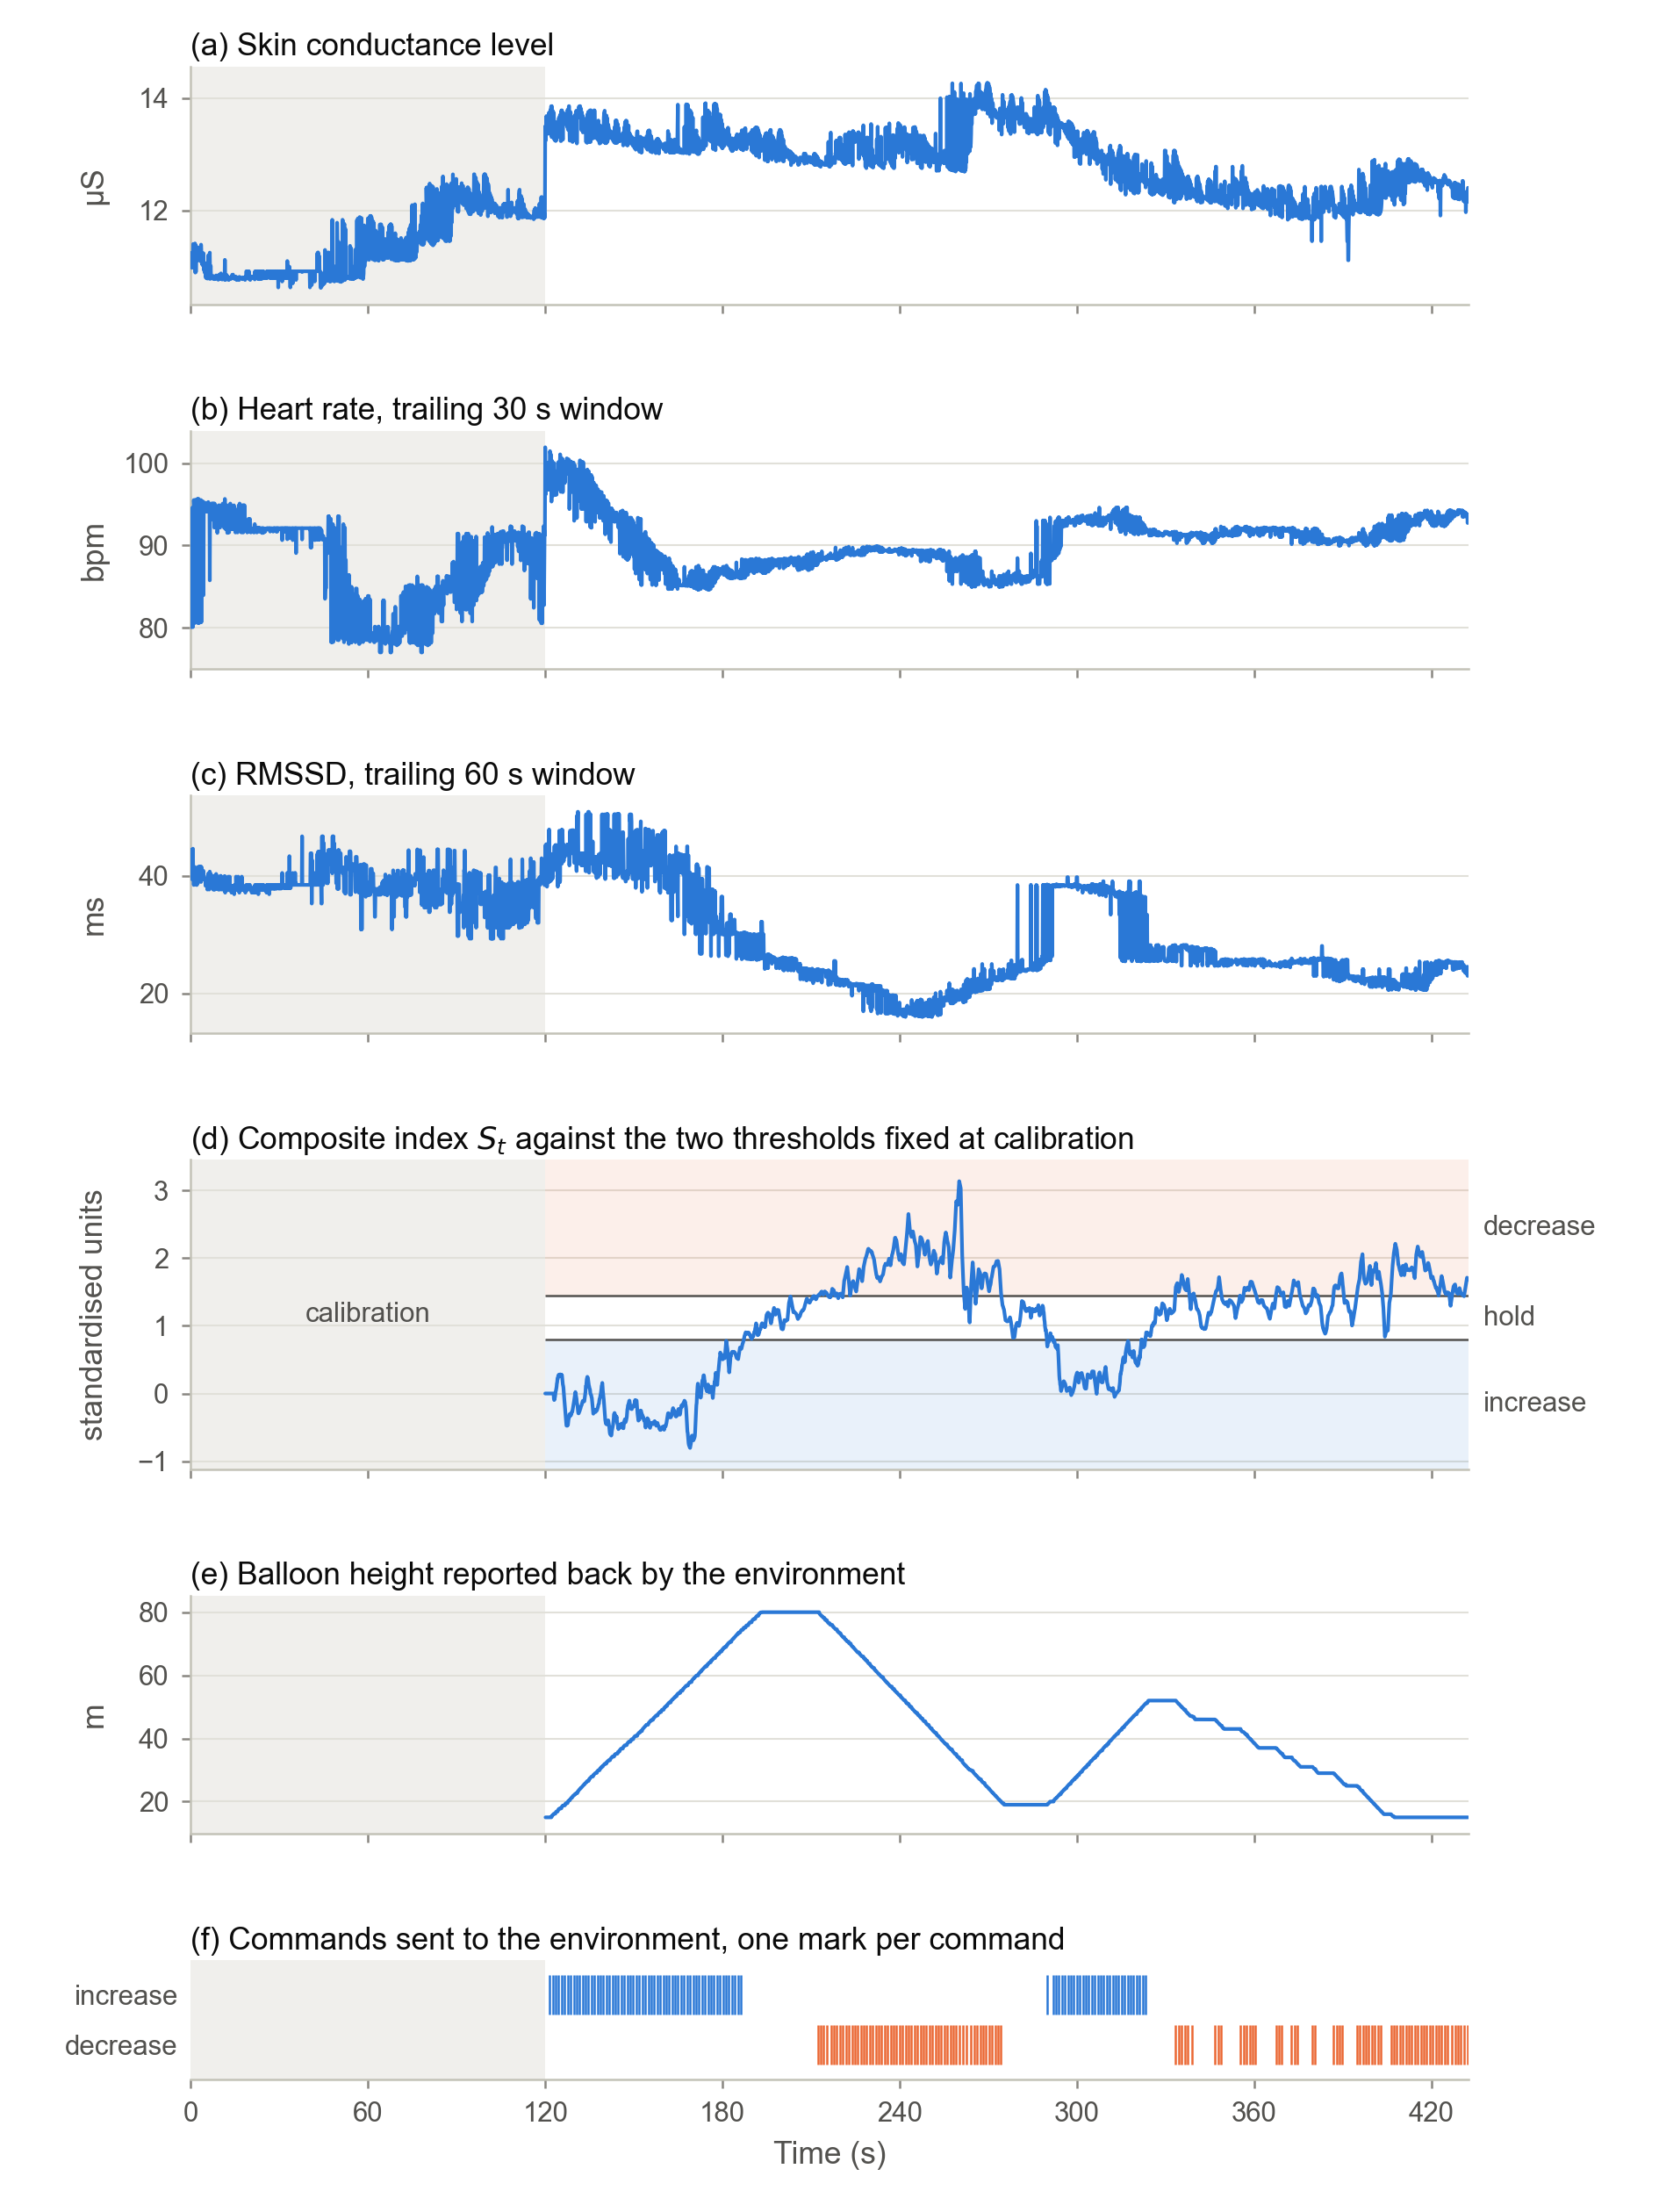
\includegraphics[width=0.82\linewidth]{07-session-overview.png}%
    }{%
        \fbox{\parbox{0.8\linewidth}{\centering
            \vspace{2cm}
            [Upload 07-session-overview.png next to this file]
            \vspace{2cm}
        }}%
    }
    \caption{One recorded session in the height environment. From the
    top: skin conductance, heart rate and RMSSD through calibration
    (shaded) and run; the composite index against the two thresholds
    fixed at the end of calibration; the balloon height reported by the
    environment; and every command sent.}
    \label{fig:session}
\end{figure}

\section*{Contributions and implications}

The contribution is the framework itself: an apparatus, a calibration
procedure, a decision rule and a session record, specified closely
enough to be reproduced. Because measurement is separated from
presentation, one calibrated index can drive any environment that
implements the four-command interface, and environments can be compared
on identical instrumentation and arithmetic. For HCI research and
practice the work offers an inspectable pattern for physiology-driven
adaptation in immersive systems, together with the safeguards such
adaptation requires: thresholds grounded in each participant's resting
physiology, gating and rate limiting of commands, suspension of control
when the signal is lost, and a complete log that lets every adaptive
decision be audited afterwards.

\begin{thebibliography}{10}
\small

\bibitem{rothbaum1995}
B.~O. Rothbaum, L.~F. Hodges, R.~Kooper, D.~Opdyke, J.~S. Williford and
M.~North, ``Effectiveness of computer-generated (virtual reality) graded
exposure in the treatment of acrophobia,'' \emph{American Journal of
Psychiatry}, vol.~152, no.~4, pp.~626--628, 1995.

\bibitem{freeman2018}
D.~Freeman, P.~Haselton, J.~Freeman, B.~Spanlang, S.~Kishore, E.~Albery,
M.~Denne, P.~Brown, M.~Slater and A.~Nickless, ``Automated psychological
therapy using immersive virtual reality for treatment of fear of heights:
a single-blind, parallel-group, randomised controlled trial,'' \emph{The
Lancet Psychiatry}, vol.~5, no.~8, pp.~625--632, 2018.

\bibitem{moldoveanu2023}
A.~Moldoveanu, O.~Mitru\c{t}, N.~Jinga, C.~Petrescu, F.~Moldoveanu,
V.~Asavei, A.~M. Anghel and L.~Petrescu, ``Immersive phobia therapy
through adaptive virtual reality and biofeedback,'' \emph{Applied
Sciences}, vol.~13, no.~18, art.~10365, 2023.

\bibitem{kritikos2021}
I.~Kritikos, G.~Alevizopoulos and D.~Koutsouris, ``Personalized virtual
reality human-computer interaction for psychiatric and neurological
illnesses: a dynamically adaptive virtual reality environment that
changes according to real-time feedback from electrophysiological signal
responses,'' \emph{Frontiers in Human Neuroscience}, vol.~15,
art.~596980, 2021.

\bibitem{mahmoudinejad2021}
A.~Mahmoudi-Nejad, ``Automated personalized exposure therapy based on
physiological measures using experience-driven procedural content
generation,'' in \emph{Proc.\ AAAI Conference on Artificial Intelligence
and Interactive Digital Entertainment}, vol.~17, no.~1, pp.~232--235,
2021.

\bibitem{wriessnegger2026}
S.~C. Wriessnegger, S.~Kiatthaveephong, M.~Leitner and K.~Kostoglou,
``VRSPi: towards a neuroadaptive VR exposure therapy system for spider
phobia,'' \emph{Frontiers in Human Neuroscience}, vol.~20, art.~1717588,
2026.

\bibitem{kothe2025}
C.~Kothe, S.~Y. Shirazi, T.~Stenner, D.~Medine, C.~Boulay, M.~I.
Grivich, F.~Artoni, T.~Mullen, A.~Delorme and S.~Makeig, ``The Lab
Streaming Layer for synchronized multimodal recording,'' \emph{Imaging
Neuroscience}, vol.~3, art.~IMAG.a.136, 2025.

\bibitem{taskforce1996}
Task Force of the European Society of Cardiology and the North American
Society of Pacing and Electrophysiology, ``Heart rate variability:
standards of measurement, physiological interpretation, and clinical
use,'' \emph{European Heart Journal}, vol.~17, no.~3, pp.~354--381,
1996.

\bibitem{boucsein2012}
W.~Boucsein, \emph{Electrodermal Activity}, 2nd~ed. New York: Springer,
2012.

\bibitem{makowski2021}
D.~Makowski, T.~Pham, Z.~J. Lau, J.~C. Brammer, F.~Lespinasse, H.~Pham,
C.~Sch\"olzel and S.~H.~A. Chen, ``NeuroKit2: a Python toolbox for
neurophysiological signal processing,'' \emph{Behavior Research Methods},
vol.~53, no.~4, pp.~1689--1696, 2021.

\end{thebibliography}

\end{document}
